\section{问题一分析与求解}
\subsection{相关性分析}\label{问题一分析}

本节首先使用Pearson correlation,初步分析各参数对AP发送机会(seq\_time)的影响,为预测模型做准备。(数据来源:第4节预处理后的训练集)。


\begin{equation}
	\small
	\rho_{X, Y} = \frac{\operatorname{cov}(X, Y)}{\sigma_{X} \sigma_{Y}} = \frac{E(X Y) - E(X) E(Y)}{\sqrt{E(X^{2}) - E^{2}(X)} \sqrt{E(Y^{2}) - E^{2}(Y)}}
\end{equation}


% TODO: \usepackage{graphicx} required
\begin{figure}[H]
	\centering
	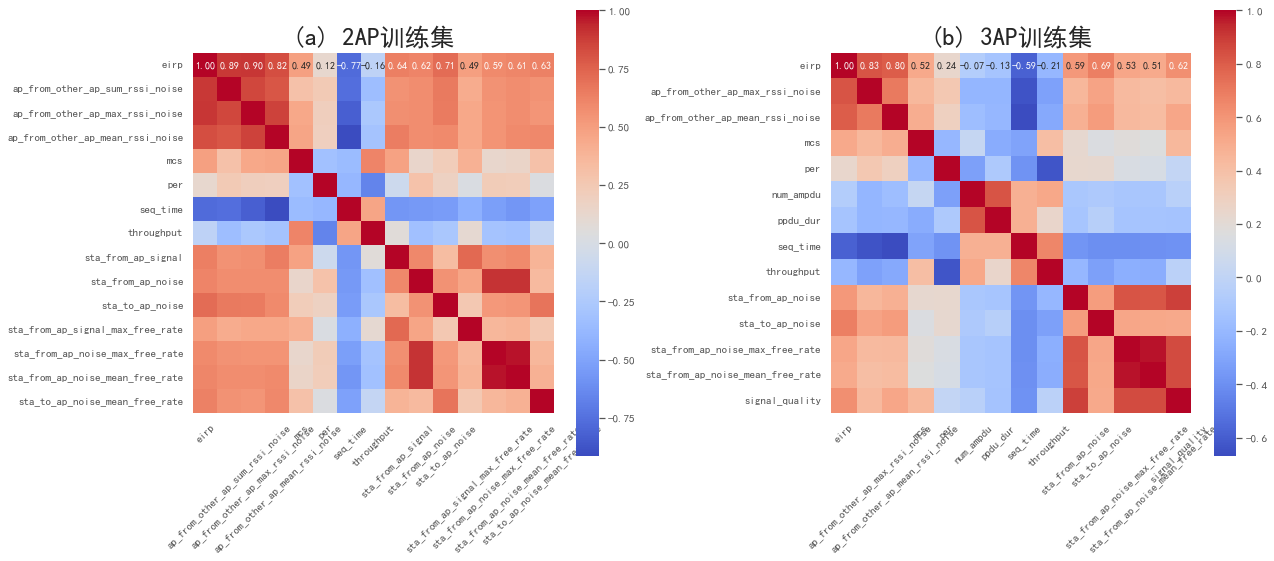
\includegraphics[width=1\linewidth]{figures/问题一热力图}
	\caption{参数相关性热力图}
	\label{fig:}
\end{figure}


如图所示,本节分析了在2AP和3AP训练集中,各参数与目标变量seq\_time之间的相关性。通过计算相关性,能够识别出对seq\_time影响显著的特征,并对其影响强弱进行排序。如表5.4所示。

\begin{longtable}{ccc}
	\caption{seq\_time影响强弱相关性(部分)}\\
	\hline
	\textbf{变量名} & \textbf{2AP} & \textbf{3AP} \\ 
	\hline
	throughput                          & 0.467841      & 0.660084      \\
	MCS                                & -0.353371     & -0.314458     \\
	per                                & -0.384524     & -0.385909     \\
	sta\_from\_ap\_signal\_max\_free\_rate & -0.430447     & -            \\
	sta\_to\_ap\_noise\_mean\_free\_rate & -0.513676     & -            \\
	sta\_from\_ap\_noise\_max\_free\_rate  & -0.528735     & -0.400428     \\
	sta\_to\_ap\_noise                    & -0.543609     & -0.404161     \\
	sta\_from\_ap\_noise                  & -0.558357     & -0.374620     \\
	sta\_from\_ap\_signal                 & -0.570747     & -            \\
	sta\_from\_ap\_noise\_mean\_free\_rate & -0.572061     & -0.396948     \\
	ap\_from\_other\_ap\_sum\_rssi\_noise & -0.761089     & -            \\
	eirp                               & -0.774949     & -0.585820     \\
	ap\_from\_other\_ap\_max\_rssi\_noise & -0.826892     & -0.634508     \\
	ap\_from\_other\_ap\_mean\_rssi\_noise & -0.912509     & -0.666785     \\ 
	\hline
\end{longtable}

1. 强影响因素:throughput在两类训练集下均为最高的正相关;多个变量(如 MCS、per 和 eirp)对seq\_time的影响均显著,表明了它们在预测seq\_time的重要性。

2. 负相关因素:eirp 和 RSSI 相关的变量均表现出较大的负相关;

3. 共性:在对2AP和3AP训练集的比较中,我们发现参数与seq\_time之间的关系呈现出一些共性,主要表现在以下几个方面:

\begin{itemize}
	\item 多数与RSSI相关的参数(如 ap\_from\_other\_ap\_mean\_rssi\_noise )在两个训练集中均表现出较高的负相关性。这表明信号的噪声和质量对发送数据帧序列的总时长(seq\_time)具有重要影响。
	\item 除RSSI相关参数外,eirp(AP的发送功率)在两个训练集中显示出显著的负相关性。
\end{itemize}


4.结论:尽管与RSSI相关的参数在影响seq\_time方面表现出一定的相关性,然而这些参数不足以支持训练高效的seq\_time预测模型,主要原因在于:

\begin{itemize}
	\item RSSI作为信号强度的度量,其值可能会受到环境干扰的极大影响,导致其对于模型学习的可预测性差。
	\item 相关性虽然显示出一定的影响,但并不能直接作为因果关系的依据。高相关性不一定意味着高因果解释力。
	\item 训练集中,与RSSI相关的参数多达20条及以上,数据维度过高可能导致过拟合及计算效率低下。
\end{itemize}

因此,有必要针对 RSSI 的相关参数进行进一步的提取和选择,并重新对RSSI进行特征构建,以提高预测模型的学习特征能力,通过计算和引入更具解释性的特征来增强模型的表达能力,将对模型的有效性和可预测性有积极影响。


\subsection{特征构建}


\subsubsection{信干噪比}

在传输过程中,信干燥比SINR可以代表着信号中所承载有效信息的比例,参考(4.1)



在公式中,由于训练集没有收集到信号或是干扰与噪声的功率大小,而RSSI一般以dBm(分贝毫瓦)表示,是接收端感知的信号强度。因此,实际上已经是信号功率的一个直接度量,所以本文在计算SINR时,由于RSSI是以功率的对数为基准的数量关系,故本文利用RSSI之间的差值来近似表示SINR。公式如下:


\begin{equation}
	RSSI_i-RSSI_j\lg \left( P_i \right) -\lg \left( P_j \right) =\lg \left( \frac{P_i}{P_j} \right) \frac{P_i}{P_j}
\end{equation}

由题可知,计算SINR的情况分为三种,故需要通过数据中AP与AP之间、AP与STA之间,STA与STA之间传输的RSSI数值大小来区分此次传输属于同步传输、异步传输还是混合传输。

\begin{table}[H]
	\centering
	\caption{不同传输形式下的RSSI监听情况}
	\begin{tabular}{@{}cccccc@{}} % 修改列数为6
		\toprule
		\textbf{类别序号} & \textbf{\shortstack{AP与AP \\ 监听RSSI}} & \textbf{\shortstack{关联AP与STA \\ 监听RSSI}} & \textbf{\shortstack{邻区AP与STA \\ 监听RSSI}} & \textbf{\shortstack{STA与STA \\ 监听RSSI}} & \textbf{传输形式} \\ \midrule
		1 & 较低 & 较高 & 较低 & 较低 & 同步传输 \\
		2 & 较低 & 较高 & 较高 & 较低 & 异步传输 \\
		3 & 时高时低 & 较高 & 时高时低 & 较低 & 混合传输 \\ \bottomrule
	\end{tabular}
\end{table}

然后通过判断不同的传输类型,可以进一步将公式(5.14)细化为:
 

\begin{equation}
	\left\{ 
	\begin{array}{l}
		\begin{matrix}
			SINR_{ST} \approx RSSI_{APtoSTA} - RSSI_N & \text{,} \text{同步传输} \\
		\end{matrix} \\[1ex]
		\begin{matrix}
			SINR_{AT} \approx RSSI_{APtoSTA} - RSSI_{neiborAPtoSTA} & \text{,} \text{异步传输} \\
		\end{matrix} \\[1ex]
		\begin{matrix}
			SINR_{MT} \approx \alpha \cdot SINR_{ST} + \left( 1 - \alpha \right) SINR_{AT} & \text{,} \text{混合传输} \\
		\end{matrix} \\
	\end{array} 
	\right.
\end{equation}


由此可以通过监听四类RSSI(sum列)来构建新的特征值SINR。

同时对于其他RSSI(max列和mean列)根据题中所提出的利用RSSI的最大值对CCA门限(PD门限与ED门限)做比较来判断数据在传输过程中是否能够正常发送并接收,利用RSSI的均值来与NAV门限做比较来判断是否要进行信道占用。所以利用这两列对不同要求门限的数值进行比较,算出其max列与mean列的信道通过率大小作为新特征值,其中CCA门限较为复杂,对于一个单元个中的数据列表中所有RSSI数值,如果小于PD门限则表示信号较弱,不能接收,若处于PD与ED门限之间,则认为它有$\beta_1$的概率携带PHY的preamble前导序列头,则端口识别为同频下的信号,这时候需要对PD门限进行比较,但他的RSSI处在PD和ED之间,则故有$\beta_1$的概率可以判断为信道繁忙,则代表信号不会收到新的数据传输干扰,同理在超过ED门限的RSSI中,有$\beta_2$的概率可以正确识别判断为信号传输判断信道繁忙,则也会成功通过信道传输。



\subsubsection{信号质量}



信号质量通常通过接收到的信号强度来衡量。因此,RSSI 值越高,表示信号质量越好。为了综合考虑来自不同 AP 的信号质量。本文对于STA端口,在收到AP的信号后,不论是两个AP的基本服务集还是三个AP的基本服务集,对STA收到的AP端口的信号进行加权平均处理,使用公式(4.7)计算得到一个综合的信号质量指标。




\subsection{模型建立与求解}

针对问题一,本文采用Stacking集成学习模型,将梯度提升学习算法,随机森林,支持向量回归以及线性回归四类算法结合起来。原因如下:

1.本题的训练集特征维度高,单一模型无法充分捕捉数据中的复杂关系。

2.训练集具有复杂性和多样性,单一模型无法有效捕捉所有的数据特征。

3.训练集样本有限,简单模型会导致高偏差,而复杂模型会造成过拟合。

4.Stacking的主要目的是提高模型的准确性和鲁棒性,特别适用于本题对准确性要求极高的场景


% TODO: \usepackage{graphicx} required
\begin{figure}[H]
	\centering
	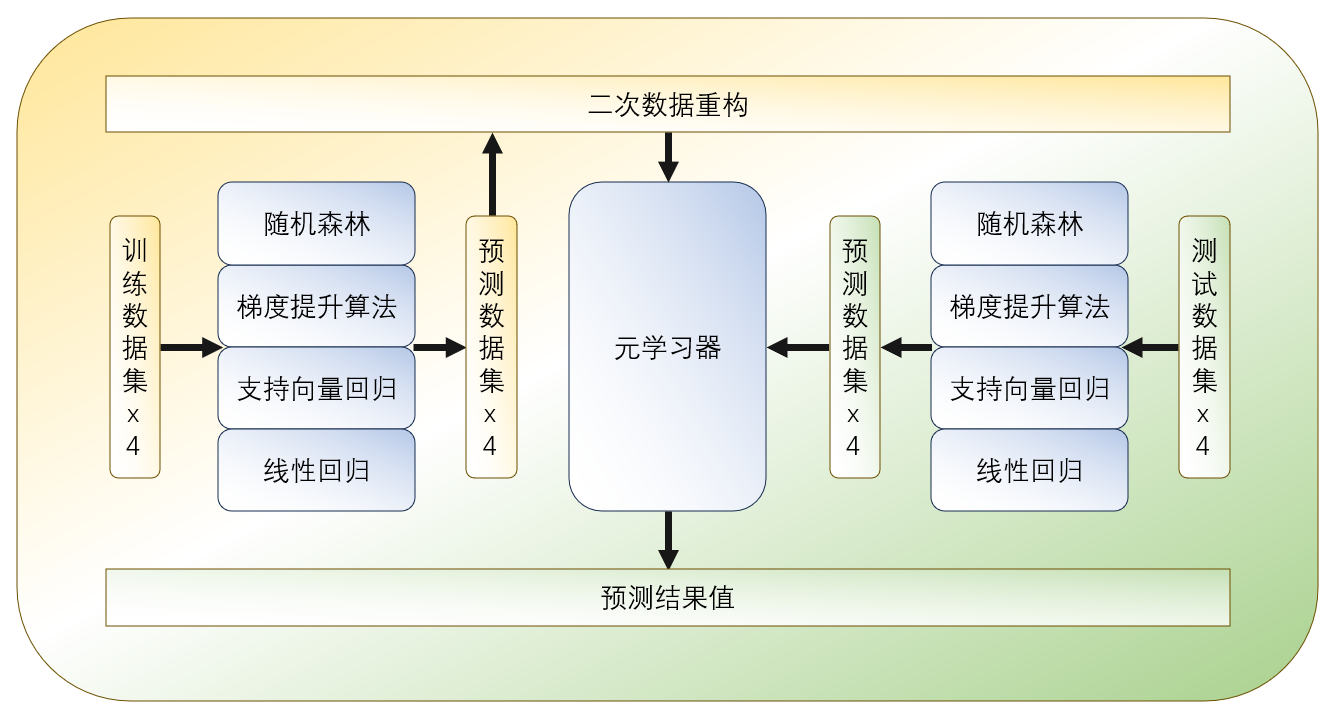
\includegraphics[width=0.7\linewidth]{figures/stacking}
	\caption{Stacking集成学习流程图}
	\label{fig:Stacking集成学习流程图}
\end{figure}

如图5.6所示,本文先将训练集放入多个基学习器中进行训练,将第一次预测的值以及训练集的目标值作为输入与输出进行数据的二测重构,放入元学习器中进行训练;测试集的特征值让四个基学习器中预测的值作为元学习器的输入值进行预测,得到的最终结果即为stacking集成学习最终的预测结果。训练使用的特征值如下表所示。

\begin{table}[H]
	\centering
	\caption{特征值(部分)}
	\begin{tabular}{ccccc} % 
		\toprule
		SINR & protocol & signal\_quality &  per & eirp\\ 
		\midrule
		 30.064 & 20 & -72.2375 &  0.27 & 13 \\
		 25 & 20 & -83.975 &  0.15 & 9 \\
	 	 25 & 8 & -83.975 &  0.14 & 9 \\
		 25.6628 & 20 & -83.8 &  0.17 & 10 \\
		\bottomrule
	\end{tabular}
\end{table}

使用Python的sklearn库,构建集成学习模型,将数据集按照7:3的比例划分为训练集和测试集,然后使用网格搜索进行超参数优化,以找到性能最佳的模型参数组合,训练出最优模型,结果如下。


\begin{table}[H]
	\centering
	\caption{模型性能对比}
	\begin{tabular}{@{}ccccccc@{}}
		\toprule
		\multirow{2}{*}{Model} & \multicolumn{2}{c}{2AP} & \multicolumn{2}{c}{3AP} & \multicolumn{2}{c}{AP} \\ 
		\cmidrule{2-3}
		\cmidrule{4-5}
		\cmidrule{6-7}
		& RMSE & R² & RMSE & R² & RMSE & R² \\ 
		\midrule
		梯度提升 & 2.747696 & 0.932200 & 3.269128 & 0.926637 & 7.125881 & 0.682336 \\
		随机森林 & 2.672078 & 0.935880 & 3.216168 & 0.928995 & 6.781550 & 0.712294 \\
		支持向量回归 & 3.589683 & 0.884281 & 4.743004 & 0.845575 & 8.301113 & 0.568914 \\
		线性回归 & 3.099190 & 0.913744 & 4.347454 & 0.870258 & 9.004967 & 0.492711 \\
		集成学习 & 2.606650 & 0.938982 & 3.102912 & 0.933908 & 6.746497 & 0.715260 \\
		集成学习(优化参数) & 1.453308 & 0.981033 & 2.757210 & 0.947814 & 6.615275 & 0.726229 \\ 
		\bottomrule
	\end{tabular}
\end{table}










如表5.7所示,本文对AP个数进行分类建模(2AP和3AP),分别训练模型,同时对AP数量统一建模,以比较集成学习模型在不同样本下的模型性能。显然,对AP数量分类后,预测性能最优。经过5重交叉验证和网格搜索调参后,最优的参数组合如下表所示。

\begin{table}[H]
	\centering
	\caption{最佳得分和参数设置}
	\begin{tabular}{cc}
		\toprule
		指标 & 最佳值 \\
		\midrule
		最佳得分 (Best Score) & 9.77534051567329 \\
		学习率 (learning\_rate) & 0.3 \\
		基学习器数量 (n\_estimators) - 梯度提升 & 200 \\
		最大深度 (max\_depth) - 随机森林 & 5 \\
		基学习器数量 (n\_estimators) - 随机森林 & 200 \\
		惩罚参数 (C) - 支持向量回归 & 10 \\
		核函数 (kernel) - 支持向量回归 & `rbf' \\
		\bottomrule
	\end{tabular}
\end{table}





% TODO: \usepackage{graphicx} required
\begin{figure}[H]
	\centering
	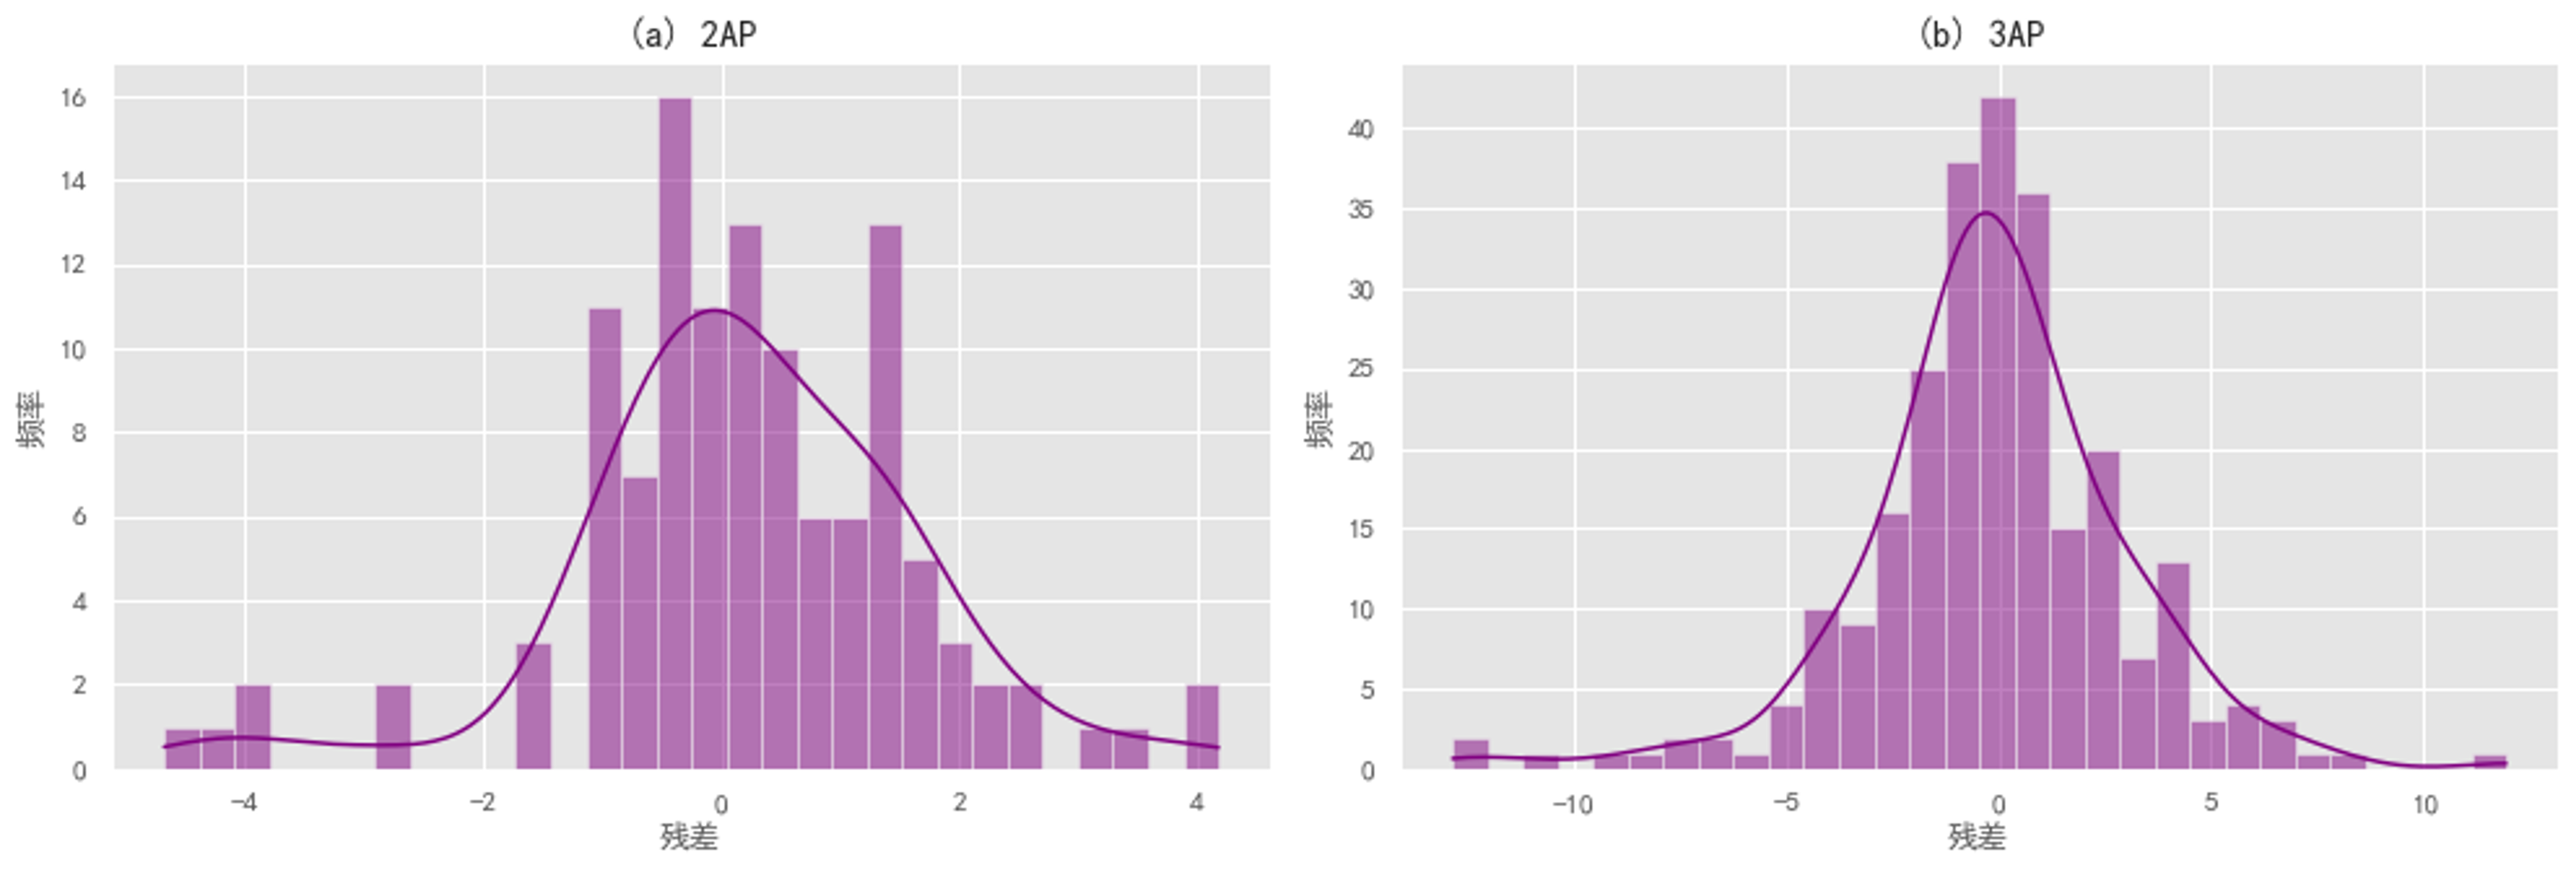
\includegraphics[width=0.9\linewidth]{figures/2ap和3ap残差图}
	\caption{Stacking模型残差分布图}
	\label{fig:2ap3ap}
\end{figure}


% TODO: \usepackage{graphicx} required
\begin{figure}[H]
	\centering
	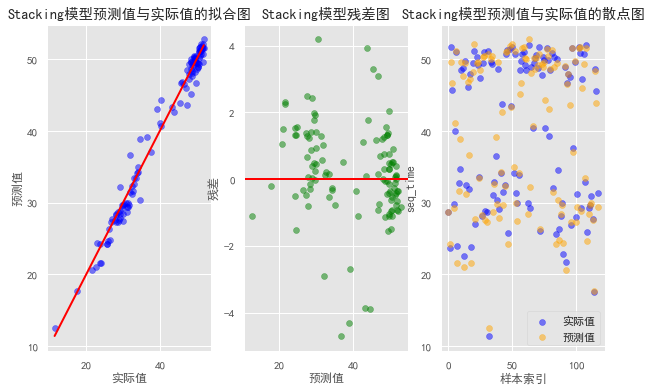
\includegraphics[width=0.8\linewidth]{figures/2ap结果}
	\caption{Stacking模型预测图}
	\label{fig:2ap}
\end{figure}



如图所示,对于2AP预测模型,残差主要分布在[ -2,+2 ]之间,测试集的平均绝对误差(MSE)为1.05,决定系数${R}^{2}$为0.98,模型预测精度较高;对于3AP预测模型,残差主要分布在[ -5,+5 ]之间,测试集的平均绝对误差(MSE)为1.84,决定系数${R}^{2}$为0.95,模型预测精度也较高,可以实现对seq\_time的高精度预测。
